\chapter{Case study}
\label{ch3}
This chapter provides the information about the use case studied. In particular, the description of the MV Oberrhein network, an overview of the SimBench database and how the time series are selected.


\section{MV Oberrhein network}
\label{sec:3mvon}
The thesis is developed in Pandapower, an open-source and popular Python library that makes it easy when working with power networks. \\
Pandapower has many features, some of them are reported here:
\begin{itemize}
    \item Every element in Pandapower (load, generator, ...) is considered as a Pandas' data frame that holds all parameters for a specific component. This implementation makes it possible to add custom columns without influencing the Pandapower functionality.
    \item It allows calculating in an easy and fast way the \gls{PF}, essential for network analysis. Its \gls{PF} solver is based on the Newton-Raphson method. \\
    After the \gls{PF} computation, the results are store in another Pandas'data frame.
    \item It allows running time series simulations.
    \item It has many predefined power networks.
\end{itemize}
%https://ietresearch.onlinelibrary.wiley.com/doi/epdf/10.1049/iet-gtd.2019.1602
Among all the power networks available in the Pandapower library, the one used for these experiments is the MV Oberrhein network. MV Oberrhein is a real distribution located at Upper Rhine (in German:  Oberrhein),  Germany. This network is a generic 20 kV power system serviced by two 25 MVA HV/MV transformer stations. The network supplies 141 HV/MV substations and 6 MV loads through four MV feeders. The network layout is meshed, but the network operates as a radial network with some open sectioning points, i.e., redundant lines/cables. This is common in real networks: they are usually meshed, but they operate in a radial way.\\
The grid also includes geographical information of lines and buses and is assembled from openly available data \cite{pandapower,mv_ob}.  \\

The representation of the network is presented in \ref{fig:MVober}. The blue dots represent the buses where load and/or generators are connected to, and the yellow squares represent the HV/MV substations.
\begin{figure}[H]
\centering
    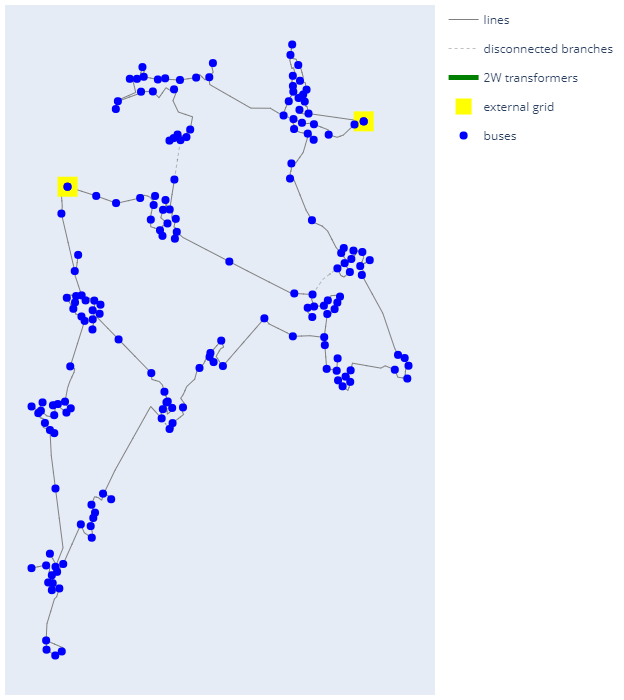
\includegraphics[height=.35\linewidth]{images/MVOberr/MVOberr.PNG}
    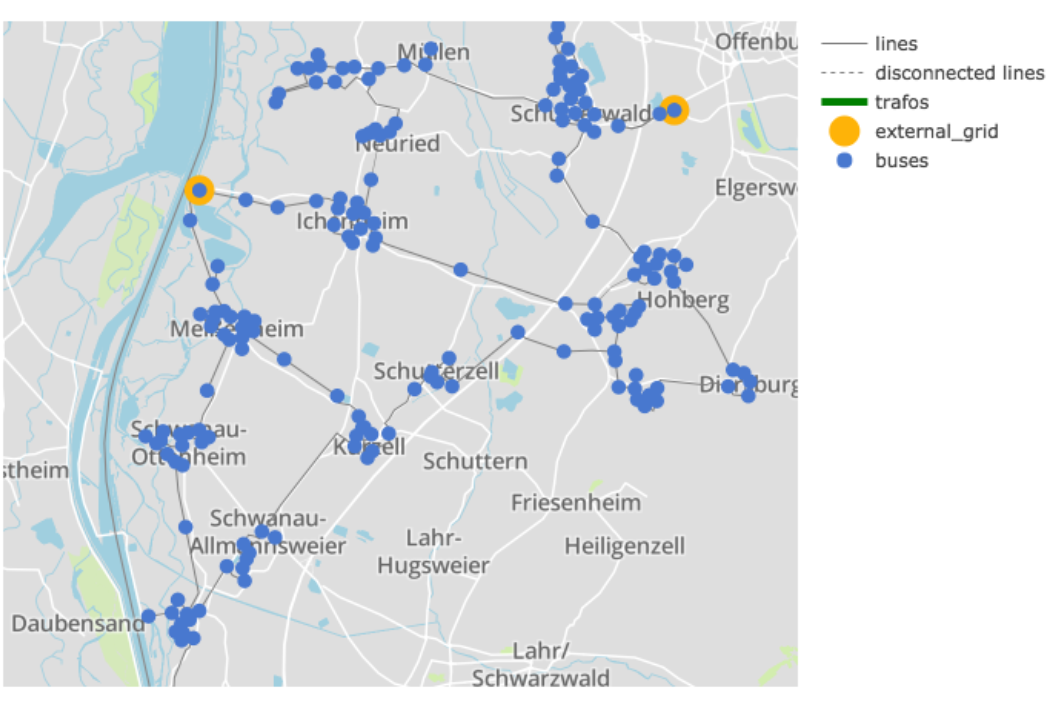
\includegraphics[height=.35\linewidth,width=.35\linewidth]{images/MVOberr/MVOberrMap1.PNG}
\caption[MV Oberrhein network]{MV Oberrhein network from Pandapower. Representation plot on the left and geographical plot on the right.}
\label{fig:MVober}
\end{figure}

\noindent To simplify the situation, the network can be divided in 2 independent parts:
% [\href{https://kobra.uni-kassel.de/bitstream/handle/123456789/12005/kup_9783737608725.pdf?sequence=1&isAllowed=y}{ref}].

\begin{figure}[H]
\centering
\subfloat[\label{fig:MVObbA}]
    {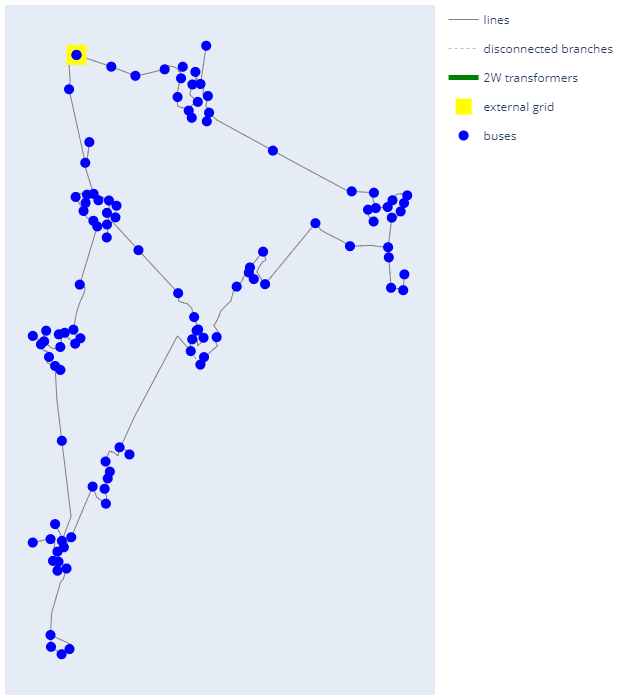
\includegraphics[width=0.3\linewidth]
    {images/MVOberr/MVOberr_half2.png}}
\subfloat[\label{fig:MVObbB}]
    {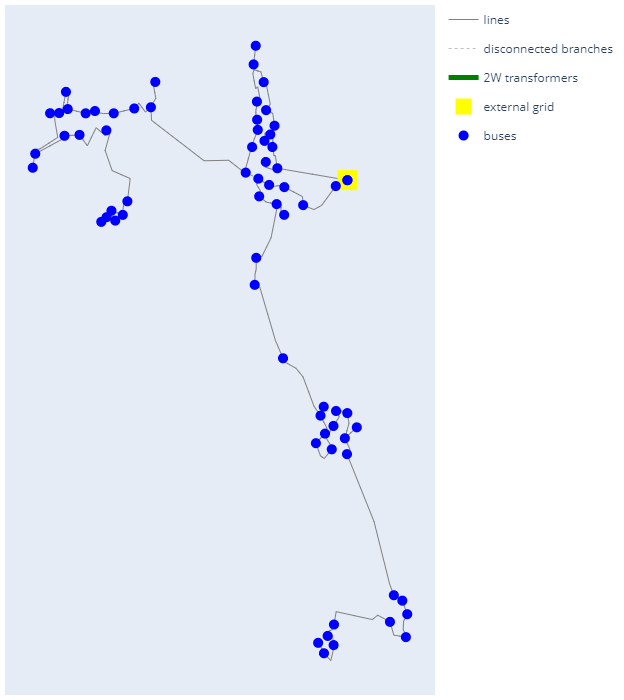
\includegraphics[width=0.3\linewidth]
    {images/MVOberr/MVOberr_half1.png}}
\caption[MV Oberrhein network division]{MV Oberrhein network division in the two parts, each with its own external grid.}
% \label{fig:MVoberdiv}
\end{figure}

The network used in this thesis is the one showed in figure \ref{fig:MVObbB}. The network consists of: one external grid, one transformer, 70 buses, 61 loads and 60 generators.

% Power networks generally operate radially as a tree, with the root the substation. The root substation can be seen as a slack bus, where the voltage magnitude \gls{V} and the phase angle \gls{angleV} are considered constants.
% Several variables are associated with each bus $n \in \mathcal{N}$: a bus voltage $\mathcal{V}_i$, a bus current injection $I_i$, an active power injection $P_i$ and reactive power injection $Q_i$. 
%The complex powers $S_i$, $S_d$ $\in \mathbb{C}$ injected into the network at bus $i$, or device $d$, can be obtained by the relation $S_i = P_i + \mathbf{i}Q_i$ or $S_d = P_d + \mathbf{i}Q_d$. \\
%Similarly, variables $I_{ij}$, $P_{ij}$, $Q_{ij}$ and $S_{ij}$ refer to the direct flow of the quantities in branch $e_{ij}$ as measured at bus $i$ \cite{gym-anm}.\\


\section{SimBench database}
\label{sec:3sd}
The time series used is taken from the SimBench database. This database refers to some real distribution networks in Germany of the year 2016. SimBench includes multiple time series for one year with 15 min resolution for loads, generators and storage units. The time series were grouped by element type, reducing the total number of required time series to a reasonable number, while retaining the possibility to model individual nominal power \cite{Simbenchds0}. All active power values are normalised to the maximum active power value.\\

Power utilities commonly use generic load profiles to group commercial customers with similar load shapes into categories or standard load profiles (\glspl{SLP}). \\
The most commonly used profile sets are developed by the German Association of Energy and Water Industries (\gls{BDEW}). It comprises eleven aggregated profiles, one for residential consumers, three for agricultural, and seven for commercial consumers with different opening hours. They are differentiated into workdays, Saturdays and Sundays as well as three seasonal categories winter, summer, and transitional. The set also includes two profiles for street lightning and band load. \\
The generation time series for photovoltaics (\glspl{PV}) and wind energy dataset are generated using an agent-based simulation tool for optimised grid expansion planning: SIMONA. SIMONA's power plant models receive real weather data of Germany from the German Weather Service in 2011 for Wind and 2012 for \gls{PV} time series as input data. \\
For 2011 and 2012 generation data, the time axis is adjusted to 2016 by shifting days so that they correspond to the nearest weekday\cite{Simbenchds1}.\\

\begin{figure}[h]
\centering
    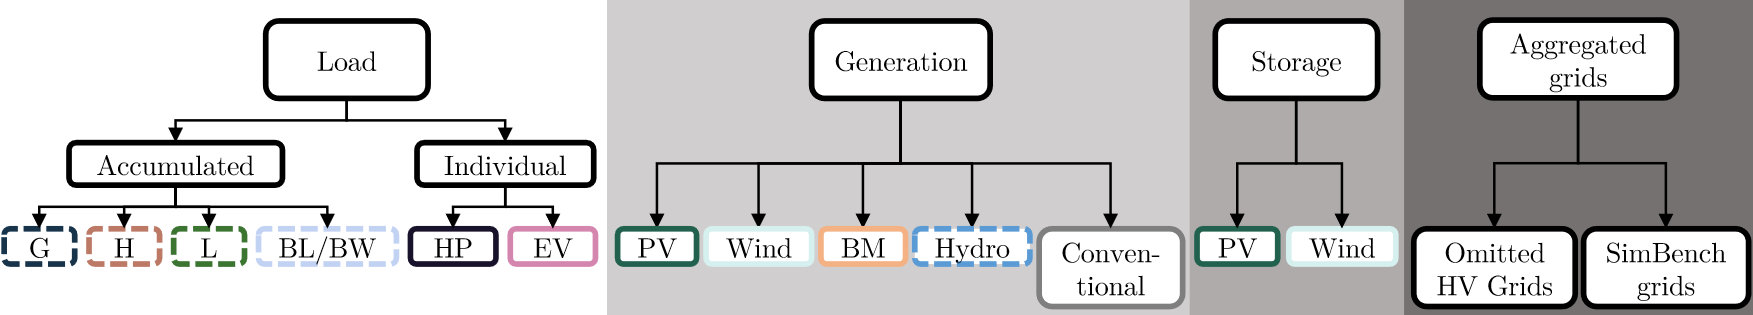
\includegraphics[width=.95\linewidth]{images/MVOberr/SimBench time series types.PNG}
\caption[SimBench time series type]{Overview of the SimBench time series type.}
\label{fig:SBtimeseriestype}
\end{figure}

The load time series were distinguished between real measured accumulated, highlighted with a dash, and simulated individual consumers, marked with a solid frame in figure \ref{fig:SBtimeseriestype}. \\



\section{Time series selection}
\label{sec:3tss}
Some time series from the SimBench database are taken to adapt to the number of loads and \glspl{DER} of the MV Oberrhein network in consideration. \\

As said, each element (load or generator) falls under a specific profile type that represents the consumption or generation over time.

\begin{figure}[H]
\centering
    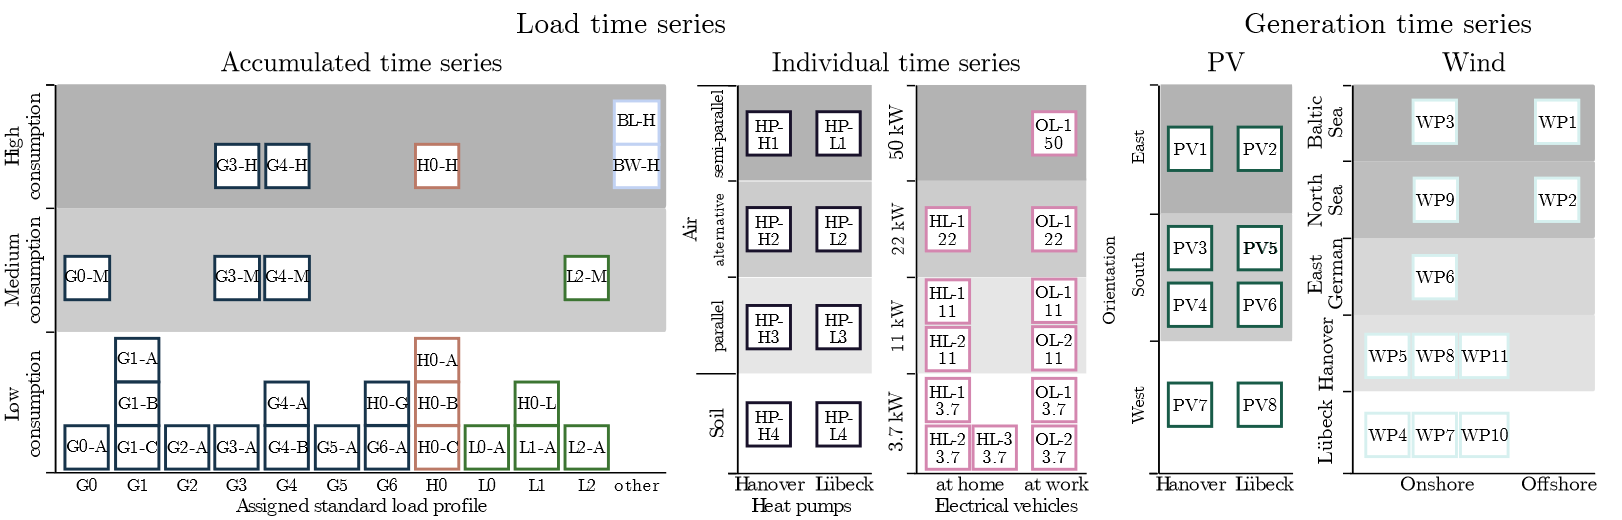
\includegraphics[width=.95\linewidth]{images/MVOberr/SimBench load and generation time series.PNG}
\caption[SimBench loads and generations standard profiles]{Loads and generations standard profiles.}
\end{figure}

In this case, the profile's types for loads and \glspl{DER} are chosen, such that every profile type is present, to have a network as close as possible to a real network. \\
The profiles' distribution in the Pandapower network is as follows:

\begin{algorithm}[h]
\State Load elements by type: \{"G0-A": 4, "G0-M": 4, "G1-A": 3, "G1-B": 3, "G1-C": 3, "G2-A": 3, "G3-A": 4, "G3-M": 3, "G4-A": 3, "G4-B": 3, "G5-A": 3, "G6-A": 3, "H0-A": 3, "H0-B": 3, "H0-C": 4, "L0-A": 3, "L1-A": 3, "L2-A": 3, "L2-M": 3\}\\

\State DER elements by type: \{"PV1": 7, "PV3": 7, "PV4": 7, "PV5": 8, "PV6": 8, "PV7": 8, "WP4": 7, "WP7": 8\}
\end{algorithm}
\noindent where the letters stand for: commercial enterprises (G), households (H) and agricultural holdings (L); with last letters -A to -C indicating low consumption and -M medium consumption customers. \\
For the \gsl{DER} devices there are photovoltaics \glspl{PV} and wind parks \glspl{WP}. It is possible to notice a bigger presence of \glspl{PV} over \glspl{WP}.\\

The loads and \glspl{DER} are chosen so that different profile types are present.

\begin{figure}[H]
\centering
    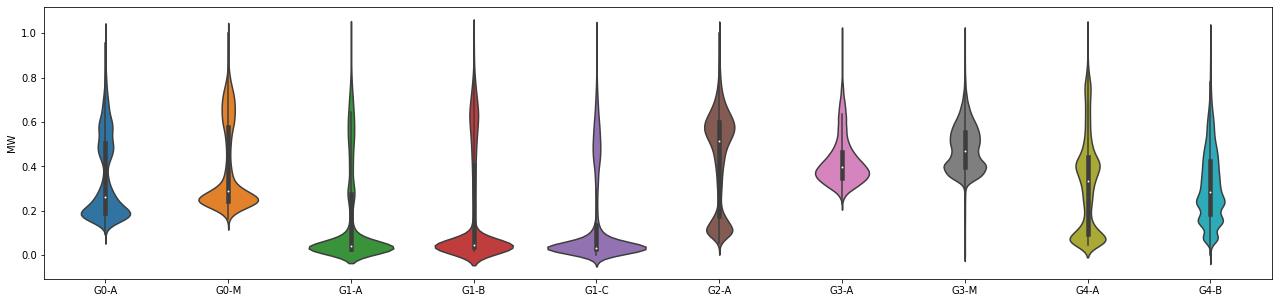
\includegraphics[width=0.95\linewidth]    {images/MVOberr/ViolinPlotLoad1.png}\\
    
    \subfloat[\label{fig:loadprofile} load profiles]            {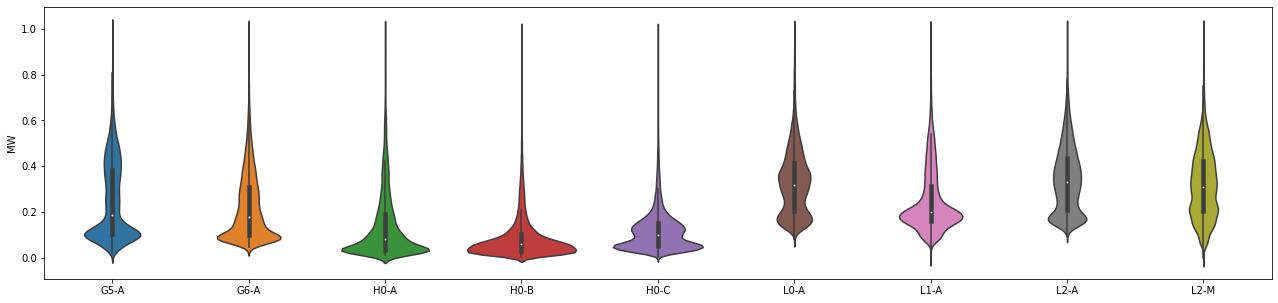
\includegraphics[width=0.95\linewidth]{images/MVOberr/ViolinPlotLoad2.png}}\\
    
    \subfloat[\label{fig:genprofile} generator profiles]    {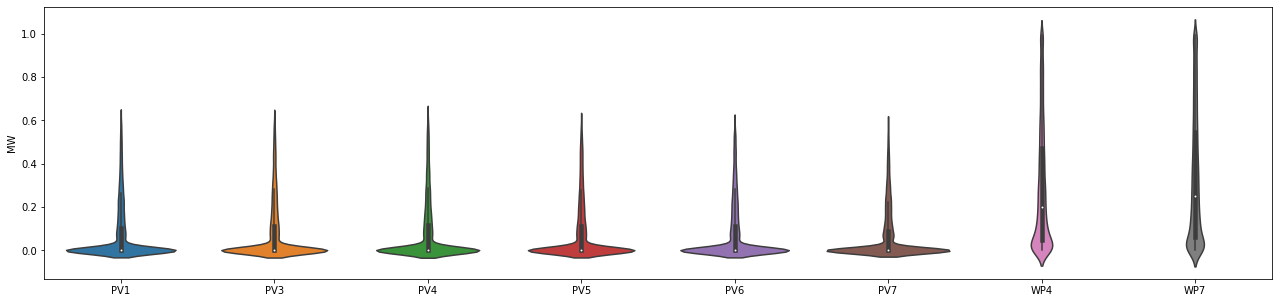
\includegraphics[width=0.95\linewidth]    {images/MVOberr/ViolinPlotRes.png}}
\caption[Violin plots of loads and generators]{Violin plots of loads and generators for each profile type.}
\label{fig:lodprof}
\end{figure}

\noindent From plots in figure \ref{fig:lodprof} it is possible to see the distribution of consumptions and generation of the different profiles.\\

Since the profiles are similar for every element of the same type, some noise is added to increase randomness. In particular, the noise added is a scaling factor in the range [0.85,1.15]. The scaling factor allows avoiding negative values in case of a value lower than 1; subtraction may result in a negative value of active or reactive power for a particular device, either load or generator. \\

It is possible to use some scaling factors to easily generate different case that can fit with the network considered. The scaling factors, chosen in this case, are:
\begin{algorithm}[h]
    \State scale\_factor\_load = 0.8
    
    \State scale\_factor\_der = 1.2
\end{algorithm}

These values are chosen to be close to the load and generation peak capacity of the MV Oberrhein network.\\

\begin{figure}[H]
\centering
    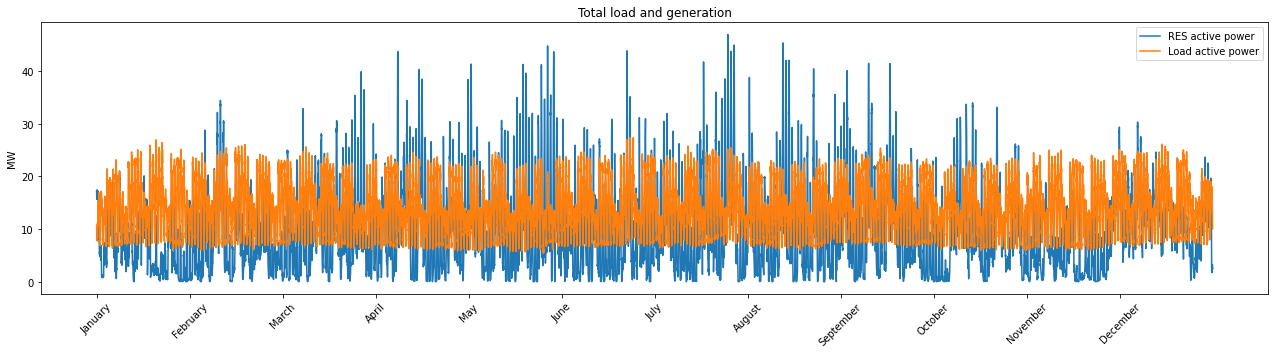
\includegraphics[width=1\linewidth]{images/MVOberr/Load&Gens.png}
\caption[Consumed and generated energy]{Sum of load energy consumption and \gls{DER} energy generation over the considered year.}
\end{figure}

The load consumption values are as a typical MV network (\cite{MVnetworks}), while the generation is higher. This case can represent a future power network when the number and the performance of \gls{DER} devices increase, so to have a generation of power higher than the demand; especially during the summer period when the consumption is lower and the generation is higher.\\
Such situations are critical for a network since the surplus energy increases the voltages at the buses that may experience voltage problems.\\


In this thesis, the network situation, in a given time step $t$, is considered critical if the voltage of at least one of the buses is out of the boundaries $V_t < v^{\text{min}}$ (under voltage) or $V_t > v^{\text{max}}$ (over voltage), where $v^{\text{min}}$ is the minimum acceptable voltage, $0.95$ \gls{pu}, and $v^{\text{max}}$ is the maximum one, $1.05$ \gls{pu}\\
\begin{figure}[H]
\centering
    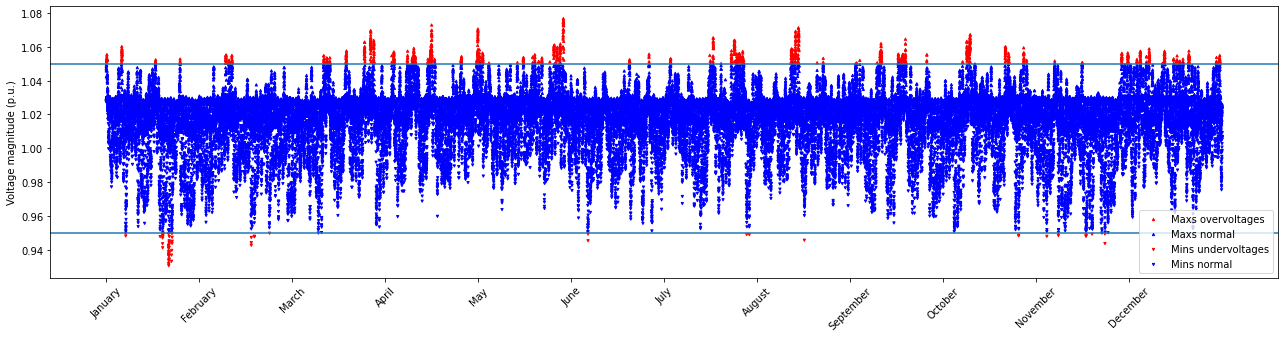
\includegraphics[width=1\linewidth]{images/MVOberr/CritialSituations.png}
\caption[Network's critical situations]{Network's over and under voltage critical situations. The two horizontal lines correspond to $v^{\text{max}}$ and $v^{\text{min}}$.}
\label{fig:ctb}
\end{figure}

In figure \ref{fig:ctb}, it is possible to see that the number of over voltages situations is low compared to the normal situations. It is possible to see that there are also few under voltage situations.\\

This concludes the part relative to aim \ref{aim1} to adapt to a real power network some realistic time series.